\documentclass[border=10pt]{standalone}
\usepackage[svgnames]{xcolor}
\usepackage{amsmath}
\usepackage{pgfplots}
\pgfplotsset{compat=newest}
\usepackage[sfdefault]{FiraSans}
\usepackage{FiraMono}
\renewcommand*\familydefault{\sfdefault}
\begin{document}
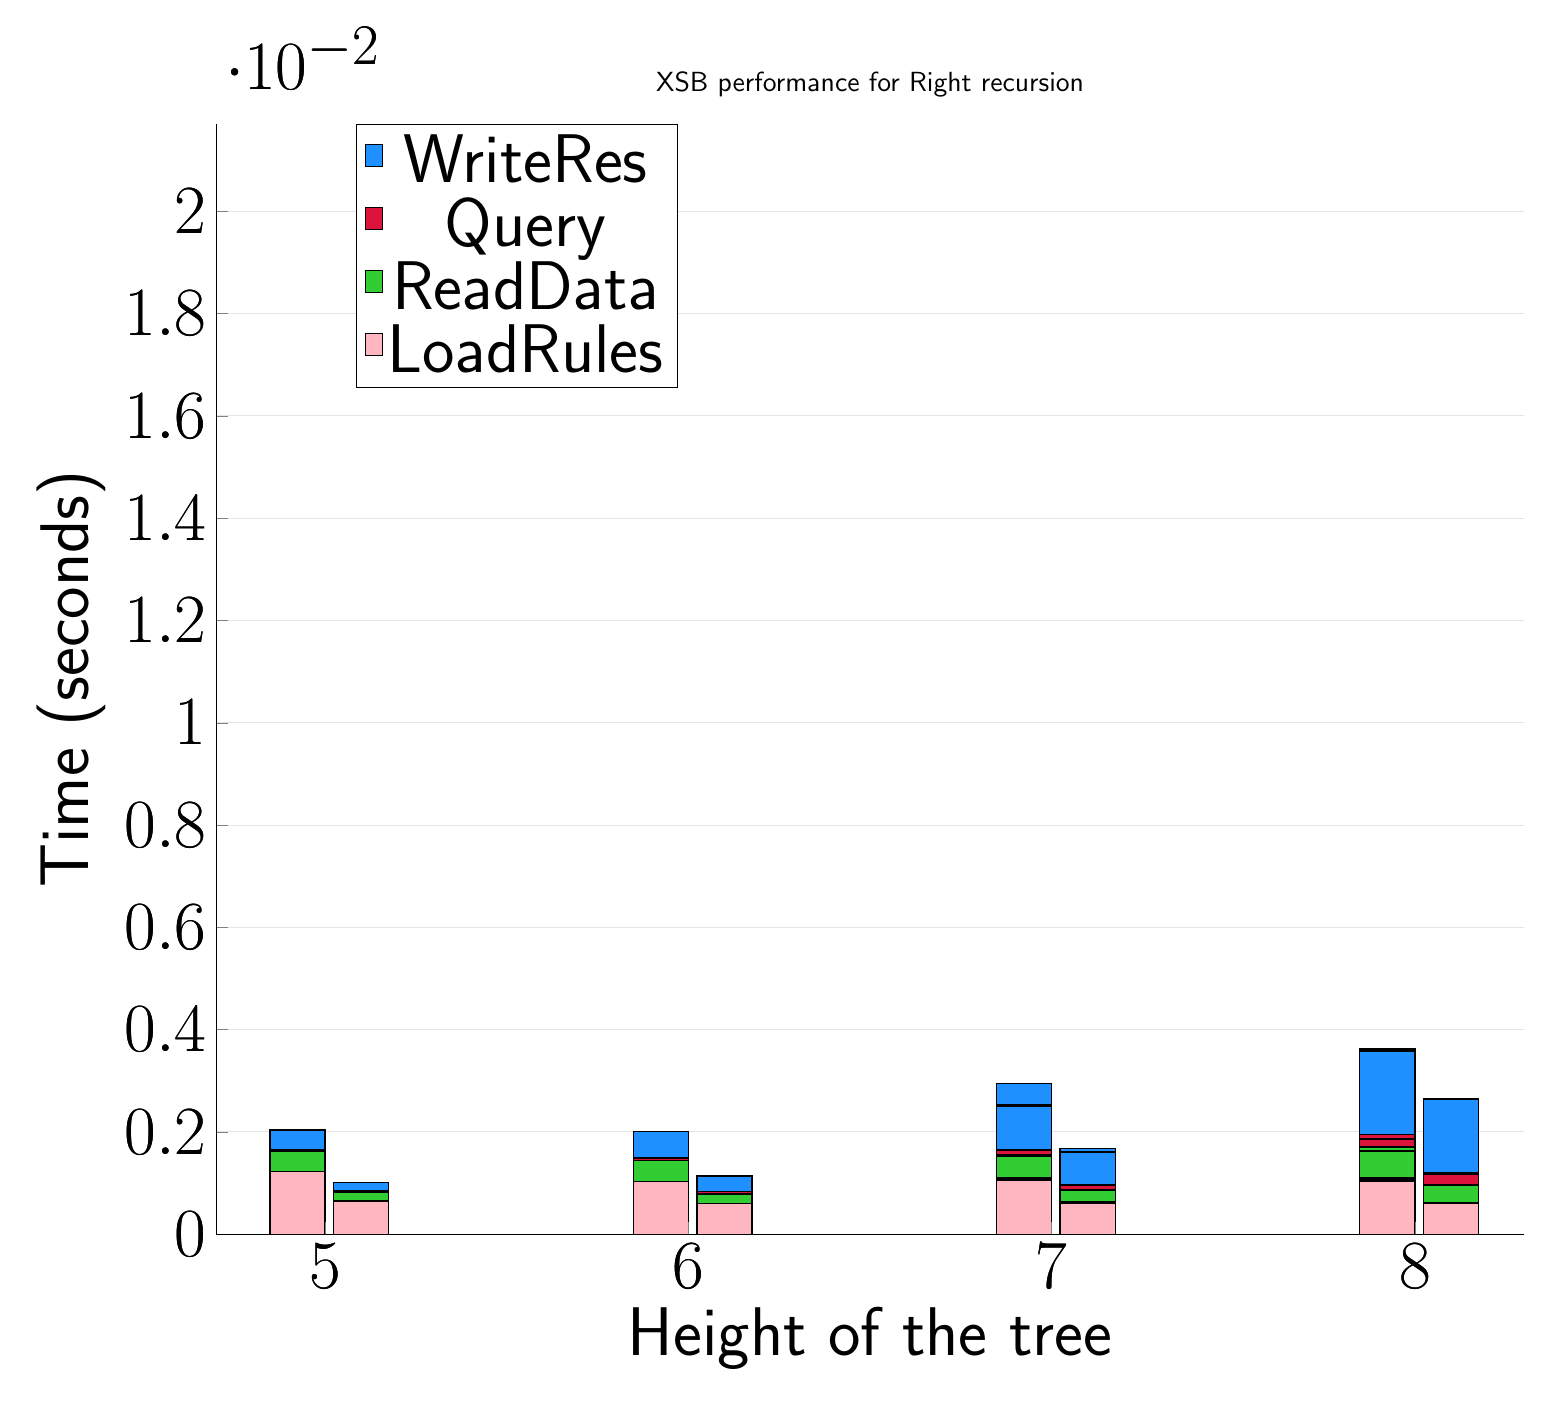
\begin{tikzpicture}
	\begin{axis}[
			ybar stacked,
			title={XSB performance for Right recursion},
			bar shift=-10pt,
			width=1.5\textwidth,
			bar width=0.7cm,
			ymajorgrids, tick align=inside,
			major grid style={draw=gray!20},
			xtick=data,
			ymin=0, ymax=0.021717853546142578,
			axis x line*=bottom,
			axis y line*=left,
			enlarge x limits=0.1,
			legend style={
					at={(0.23, 1)},
					anchor=north,
					legend columns=1,
					font=\Huge,
				},
			ylabel={Time (seconds)},
			xlabel={Height of the tree},
			label style={font=\Huge},
			tick label style={font=\Huge},
		]
		\addlegendimage{fill=DodgerBlue, draw=black, line width=0.2pt}
		\addlegendentry{WriteRes}
		\addlegendimage{fill=Crimson, draw=black, line width=0.2pt}
		\addlegendentry{Query}
		\addlegendimage{fill=LimeGreen, draw=black, line width=0.2pt}
		\addlegendentry{ReadData}
		\addlegendimage{fill=LightPink, draw=black, line width=0.2pt}
		\addlegendentry{LoadRules}
		\addplot +[fill=LightPink, draw=black, line width=0.5pt] coordinates {
				(5, 0.001227331161499022)
				(6, 0.0010321855545043935)
				(7, 0.0010548830032348628)
				(7, 0.0010687351226806628)
				(7, 0.001099085807800291)
				(8, 0.0010566949844360352)
				(8, 0.001097297668457033)
				(8, 0.001042842864990234)
			};
		\addplot +[fill=LimeGreen, draw=black, line width=0.5pt] coordinates {
				(5, 0.00038506984710693357)
				(6, 0.0004070520401000975)
				(7, 0.0004772424697875977)
				(7, 0.00046539306640624984)
				(7, 0.0004472494125366211)
				(8, 0.000565481185913086)
				(8, 0.0006067752838134767)
				(8, 0.0005995750427246094)
			};
		\addplot +[fill=Crimson, draw=black, line width=0.5pt] coordinates {
				(5, 3.4499168395996084e-05)
				(6, 5.3954124450683596e-05)
				(7, 0.0001097917556762696)
				(7, 0.00011219978332519532)
				(7, 0.0001118898391723633)
				(8, 0.00023164749145507808)
				(8, 0.0002417087554931641)
				(8, 0.00023322105407714826)
			};
		\addplot +[fill=DodgerBlue, draw=black, line width=0.5pt] coordinates {
				(5, 0.00039184093475341786)
				(6, 0.0005146741867065429)
				(7, 0.0008635044097900389)
				(7, 0.0008882284164428699)
				(7, 0.0012919902801513668)
				(8, 0.001766252517700195)
				(8, 0.00167388916015625)
				(8, 0.0017085075378417964)
			};
	\end{axis}
	\begin{axis}[
			ybar stacked,
			bar shift=13pt,
			width=1.5\textwidth,
			bar width=0.7cm,
			ymajorgrids, tick align=inside,
			major grid style={draw=none},
			xtick=data,
			ymin=0, ymax=0.021717853546142578,
			axis x line*=none,
			axis y line*=none,
			enlarge x limits=0.1,
			label style={font=\Huge},
			tick label style={font=\Huge},
		]
		\addplot +[fill=LightPink, draw=black, line width=0.5pt] coordinates {
				(5, 0.0006482000000000001)
				(6, 0.0006023000000000003)
				(7, 0.0006140000000000001)
				(7, 0.0006172999999999997)
				(7, 0.0006282999999999998)
				(8, 0.0006067999999999997)
				(8, 0.0006163)
				(8, 0.0006037000000000002)
			};
		\addplot +[fill=LimeGreen, draw=black, line width=0.5pt] coordinates {
				(5, 0.0001656000000000008)
				(6, 0.00018409999999999979)
				(7, 0.0002479000000000005)
				(7, 0.00024650000000000003)
				(7, 0.0002437000000000006)
				(8, 0.00034750000000000037)
				(8, 0.0003618999999999993)
				(8, 0.00036130000000000027)
			};
		\addplot +[fill=Crimson, draw=black, line width=0.5pt] coordinates {
				(5, 2.909999999999925e-05)
				(6, 4.959999999999997e-05)
				(7, 0.00010279999999999979)
				(7, 0.00010360000000000005)
				(7, 0.0001047999999999999)
				(8, 0.0002151000000000001)
				(8, 0.00022010000000000028)
				(8, 0.00021389999999999972)
			};
		\addplot +[fill=DodgerBlue, draw=black, line width=0.5pt] coordinates {
				(5, 0.00016390000000000084)
				(6, 0.0003033000000000003)
				(7, 0.0006450000000000001)
				(7, 0.0006495999999999999)
				(7, 0.0007010999999999999)
				(8, 0.0014631)
				(8, 0.0014464999999999997)
				(8, 0.0014653000000000005)
			};
	\end{axis}
\end{tikzpicture}

\end{document}
